%% 
%% 
%% 

\chapter{The Skill-Action (SA) Architecture: Multi-timescale
  Sequence Learning under Hierarchical Reinforcement Learning
  Framework}
\chaptermark{The Skill-Action Architecture}
\label{cha:sa_app}


Reinforcement Learning (RL) is a paradigm for imitating humans
trial-and-error learning process: RL trains an agent to maximise
rewards by taking actions in and receiving feedback from an
environment. RL has achieved human-level performance in playing
video and board games \cite{mnih2015human,silver2016mastering}.
However, while humans can abstract the hierarchical complexity of
actions through interactions with the environment and make
decisions at both macro and micro time scales, conventional RL
agents have limited abilities to solve complex tasks
\cite{daniel2016probabilistic}: they only learn the most
primitive actions and make decisions at the smallest time scale.
Hierarchical Reinforcement Learning (HRL) attempts to resolve
this gap between humans and RL by decomposing complex tasks into
a hierarchy of abstracted actions at multiple time scales.

An HRL agent typically learns abstractions of actions on two
levels: skills and primary actions. Skills are higher-level
abstracted actions. Their executions are temporally extended to a
variable amount of time. Primary actions are lower-level actions
defined by the environment. They are executed at every time step.
For example, for a humanoid robot, walking and jumping are two
abstract skills, while movements of each joint are primary
actions. One of the most promising HRL frameworks is the option
framework~\cite{sutton1999between}. The option framework has
achieved great success in representing actions at different time
scales~\cite{bacon2017option}, speeding and scaling up
learning~\cite{bacon2018temporal}, improving exploration
\cite{harb2018waiting}, and facilitating transfer learning
\cite{zhang2019dac}.

In the option framework, an option is a primary action level
sub-policy consisting of an action policy, a termination
probability, and an initiation set. A master
policy~\cite{zhang2019dac} (aka
policy-over-options~\cite{sutton1999between}) is used to compose
those options and thus is a skill-level policy. The option
framework is formulated as a Semi-Markov Decision Problem
(SMDP)~\cite{puterman2014markov}: an option sampled from a master
policy is executed through a variable amount of time (until its
termination function determines to stop). As highlighted in the
literature, the SMDP formulation has the following limitations:

\begin{enumerate}
\item Sample inefficiency \cite{zhang2019dac}: a) For policy
  gradient based algorithms, the master policy cannot be updated
  until stop. As a result, one update consumes various time steps
  of samples. b) At each time step, only one (the executed)
  option's policies can be updated.
\item Large variance
  \cite{zhang2019dac,haarnoja2018soft}: SMDP
  algorithms are notoriously sensitive to hyperparameters . Due
  to the SMDP formulation, more stable Markov Decision Process
  (MDP) policy gradient algorithms cannot be used.
\item Expensive to scale up \cite{riemer2018learning}: for $M$
  options, there are $2M$ action and termination policies. Each
  policy is a neural network that could have millions of
  parameters to train.
\end{enumerate}

To address these problems, we propose a simple yet effective MDP
implementation of the option framework, the Skill-Action (SA)
architecture. The idea behind SA originates from our new
discovery that the SMDP option framework has an MDP equivalence,
which is achieved by adding extra dependencies into the master
policy. However, those extra dependencies still prevent the
master policy from being updated at every time step. Based on
this equivalence, a ``skill policy'' which marginalizes those
dependencies away is derived and hence can be updated at each
time step.

In SA, knowledge of a skill is explicitly represented as a skill
context vector (similar to an embedding
vector~\cite{vaswani2017attention} in Natural Language Processing
(NLP) or capsule~\cite{sabour2017dynamic} in Computer Vision
(CV)): each dimension encodes a particular property of the
skill\footnote{For example, the first dimension may encode the
  orientation of a primary action. A jump skill context vector
  may have a large first dimension value which instructs the
  robot to emit primary actions vertically. A walk skill may have
  a small value and emit actions horizontally.}. The skill policy
is similar to a compatibility function: it is used to replace the
master policy and termination function while improving their
functionalities by employing the attention
mechanism~\cite{vaswani2017attention}. At each time step, the
skill policy measures the compatibility (suitability) of all
skills with the current state and the executed skill from the
last step. If the previous skill still fits the current
situation, then the skill policy tends to continue with it;
otherwise, a new skill with better compatibility will be sampled.
Unlike the option framework, which requires $M$ action policies
for $M$ skills, SA's action policy only needs one decoder to
decode any skill context vector into primary actions. With this
formulation, the entire framework is MDP-based while the skill
can still be temporally extended, and its scalability, as well as
stability, are significantly improved. % todo: reconsider
All of these design choices have precursors in the existing
literature
(HRL~\cite{sutton1999between,bacon2018temporal,zhang2019dac};
CV~\cite{kosiorek2019stacked}; NLP~\cite{vaswani2017attention}).
Our contribution is establishing them in reinforcement learning
settings.

Compared to the SMDP option framework, SA has following
advantages:

\begin{enumerate}
\item SA is more sample efficient, because a) SA is MDP
  formulated, thus sample at each time step can be used to update
  the skill policy; and b) Only one action policy decoder is
  needed. It learns to decode each dimension of the skill context
  vector at each time step whichever skill is activated;
\item SA has smaller variance, because a) The skill value upon
  arrival function (Eq.~(\ref{eq:sa_v})) is theoretically and
  empirically proven to have smaller variance than the
  conventional value function; and b) SA only needs to train two
  (skill and action) policy networks; and c) SA can employ more
  stable MDP based policy gradient algorithms (e.g.
  PPO~\cite{schulman2017proximal});
\item SA has better scalability, because a) Regardless of the
  number of skills, only two policies need to be trained; and b)
  Adding one more skill is as cheap as adding a context vector;
  % to write: disentangle; exploration; convergence speed;
  % interpretability; generalization
\item SA is more effective, because a) On infinite-horizon
  environments, SA significantly outperforms the other models;
  and b) On transfer learning environments, SA ranks the first in
  5 out of 6 environments and shows its advantages in knowledge
  reuse tasks;
\item SA has better interpretability. Unlike the option framework
  encodes abstract knowledge implicitly in action policies,
  knowledge of a skill is explicitly encoded in each dimension of
  the skill context vector.
\end{enumerate}

% Incomplete Ideas:

% 1. 问问题,要解决什么问题,在干什么
% 2. 当前sota什么状况,但是有什么问题
% 3. 你做了啥,为啥能解决问题
% 4. 你这东西有啥特点
% 5. 怎么证明这东西work
% 6. Implication 是啥

% to write: smaller variance
% to write: only one critic
% to write: deep large scale; imitation; causual relationship
% because each run variance so small; not only exploration.

% todo: skill not pg/bp; may be dynamic routing/inference/K-means
% is enough. should have much simpler design

% todo: why option converges slower than action? disentangle paper

% todo: supervised train SA first -> reinf train SA; Imitation
% Learning (dm-control CMU humanoid-v3)

% todo: formal def of the turkey: latent variables between
% actions and environment. Not observable but truly exists
% ; design an experiment to show this problem

% potential problem: currently p(o_t|s_t,o_{t-1}) is updated
% using Q(o_t,s_t). Should it be Q(o_t,s_t,o_{t-1})? Should
% R_{t+1} depends on o_{t-1}?

% Yes it should. Reason:

% No it should not. Reason: We should not model environment. This
% is model free algo. Even though in reality, environment depends
% on latent variable $o_{t-1}$ to give R_{t+1}. But we should not
% model this relationship in Q value.
% Problem: Q used to update p(o'|s',o) does not consider o
% Possible solution: instead of include o in Q, create another
% ``latent variable environment reward mechanism'' function.
% Explicitly model this latent relationship between skill and
% environment's reward

% A state-previous-skill pair.
% Previous research only consider abstract, did not demonstrate
% contextual information. Knowing which action has been done can
% help predicting whats the next move. Cooking example
% Temporal relationships between skills (skill context) has not
% been explored before. Seems to encode only one-step temporal
% relationship. In order to encode multi time steps relationships,
% one can use longer history by turning into higher order markov,
% but still markov. our proof still holds. (e.g. adding temporal
% masks back to attention, extending the decoder input vector to a
% matrix, where rows are time steps, turn it into a k-order markov
% process). Remain open for future work.

% todo: explain why attention is not the best

% idea: In order to have better temporal representation what has
% happened before, need a dynamic routing like forward algorithm
% to encode all skills have been taken in time series

% idea: maximizing reasoning entropy
% statistical random variables decreasing bias increasing variance
% reasoning variables decreasing bias decreasing variance;
% maximizing reasoning entropy

% todo: MDP equi minor contribution
% todo: Equations addressed stuffed turkey (skill policy, decoder
% in nn)
% todo: reasons for oc -> sa based on MDP:

% minor contribution: MDP
% straight forward extend to deeper layer
% NLP interface to understand/instruct which dimension encode
% what information

\section{Related Works}
\label{sec:review}

% todo: SMDP-style MDP-style
To discover options automatically, \citename{sutton1999between}
proposed Intra-option Q-learning to update the master Q value
function at every time step. However, all policies under this
formulation are approximated implicitly using the Q-learning
method. \citename{levy2011unified} proposed to unify the
Semi-Markov process into an augmented Markov process and
explicitly learn an ``overall policy'' by applying MDP-based
policy gradient algorithms. However, their method for updating
the master policy is still SMDP-style thus sample inefficient.
\citename{bacon2017option} proposed a policy gradient based
Option Critic (OC) framework for explicitly learning intra-option
policies and termination functions in an intra-option manner.
However, for the master policy's policy gradients learning, OC
still remains SMDP-style. \citename{klissarov2017learnings}
attempted to combine OC with PPO in an intra-option learning
manner (PPOC). However, as we show in
\Secref{sec:appen_hmm}, due to the SMDP formulation,
gradients they use for updating master policy are inconsistent.
\citename{zhang2019dac} reformulated the option framework into
two augmented MDPs. Under this formulation all policies can be
modeled explicitly and learned in MDP-style. However, their model
is still expensive to scale up. On single task environments, DAC
has no significant advantages over other baselines.

We must appreciate that Bacon (\cite{bacon2018temporal}; Chapter
3.6) conceptually discussed a vectorized option representation
and directly approximated the marginalized master policy.
However, no concrete formulations and policy gradients theorems
were developed in their work. \citename{daniel2016probabilistic}
proposed an MDP-formulated PGM similar to ours in
\Secref{sec:appen_oc_pgm}. However, they did not prove the
equivalence between the MDP-formulation and SMDP by employing
conditional independencies. Furthermore, their learning algorithm
is EM based while ours is policy gradient based. Our work is
motivated by capsule networks \citename{kosiorek2019stacked}
(more details in \Secref{sec:append_gist}) and is developed
independently from above literature.

With respect to optimization, \citename{zhang2019dac} pointed out
that a large margin of performance boost of DAC comes from
Proximal Policy Optimization \cite{schulman2017proximal} (PPO).
Since SA is MDP-based, it can be optimized directly with the PPO.
Recent works show that the option framework trained under
off-policy \cite{haarnoja2018soft} algorithms outperforms
on-policy methods. For instance, HO2 \cite{wulfmeier2020data}
employs a trust-region constrained off-policy algorithm and shows
that it exhibits significant advantages over on-policy methods on
both sample efficiency and performance. In this paper, we propose
SA as a general HRL framework which can be trained by both
on-policy and off-policy algorithms. Our main contribution
focuses on deriving MDPs of SA and its policy gradient theorems.
Designing off-policy algorithms for SA remains open for future
work.

Existing RL literature
\cite{hausman2018learning,li2017infogail,tirumala2019exploiting}
also uses latent variables to learn skill embeddings. Typically,
PEARL \cite{rakelly2019efficient} learns a latent context vector
for each task under the meta-reinforcement learning framework to
improve the agent's sample and transfer learning efficiency.
However, embeddings learned by RL frameworks only encode action
level abstraction while SA learns abstractions at both action and
temporal levels. It is also worth to mention that, the novel
formulation of SA establishes a strong connection to causal
reinforcement learning. When the number of skills equals one
($M=1$), SA falls back to Generalized Hidden Parameter MDPs
(GHP-MDPs) \cite{kolobov2012discovering,perez2020generalized}.
Causality properties of SA is a direction worth to be explored in
the future work.

% parameter vector in policy to encode causality between policy and
% environment properties. Causality properties of SA is a direction
% worth to be explored in the future work. There are also
% interesting attempts to introduce supervised guidance into HRL
% \cite{gupta2019relay}. With hierarchical knowledge explicitly
% represented in embedding matrix, SA provides a more efficient and
% scalable HRL model for such frameworks.
\section{MDP Equivalence to the SMDP Option Framework}
\label{sec:appen_oc_pgm}

In this section, we prove that the the conventional Semi-Markov
Decision Problem (SMDP) option framework which employs Markovian
options actually has an MDP equivalence. We first follow
\citename{bishop2006pattern}'s method and formulate the dynamics
of the option framework as an Hidden Markov Model
(HMM)~\cite{bishop2006pattern} in section~\ref{sec:appen_hmm}.
With Probability Graphical Model (PGM)~\cite{bishop2006pattern}
and its conditional independence relationships (Chapter 8.2.1
\cite{bishop2006pattern}) in hand, we then move on to prove that
MDP formulation has identical value functions
(section~\ref{sec:appen_mdp}), bellman equations as well as
intra-option policy and termination policy gradients to SMDP
formulation (section~\ref{sec:appen_mdp_grad}). To the best of
our knowledge, this is the first work discovering the option
framework's MDP equivalence and deriving the option framework
from a PGM view.

\subsection{Background: The Option Framework}
\label{sec:appen_oc_background}

\citename{sutton1999between} proposed the option framework to
demonstrate the temporal abstraction problem. A scalar
$\ro\in\sZ$ denotes the index of an option where $\sO \subseteq
\{1,2,\ldots,M\}$ and $M$ is the number of options. An Markovian
option is a triple $(\sI_{o},P_{o}(\rva|\rvs),P_{o}(\rb|\rvs))$
% $(\sI_{o_t},P_{o_t}(\rva_t,|\rvs_t),P_{o_t}(\rb_t|\rvs_t))$
in which $\sI_{o}\subseteq\sS$ is an initiation set where the
option $o$ can be initiated. $P_{o}(\rva|\rvs):\sS\rightarrow\sA$
is the intra-option policy which maps environment states
$\rvs\in\sS$ to an action vector $\rva\in \sA$.
$P_{o}(\rb|\rvs):\sS\rightarrow\sZ_2$ is a termination function
where $\rb$ is a binary random variable. It is used to determine
whether to terminate ($\rb=1$) the policy $P_{o}(\rva|\rvs)$ or
not ($\rb=0$). Conventionally, $\beta_o=P_o(\rb=1|\rvs)$. Since
an option's execution may persist over a variable period of time,
a set of options' execution together with its value functions
constitutes a Semi-Markov Decision Problem (SMDP)
\cite{puterman2014markov}. When an old option is terminated, a
new option will be sampled from the master policy
(policy-over-options) $o\sim P(o_{t+1}|\rvs_{t+1}):
\sS\rightarrow\sO$.
\begin{figure*}[th!]
  \centering
  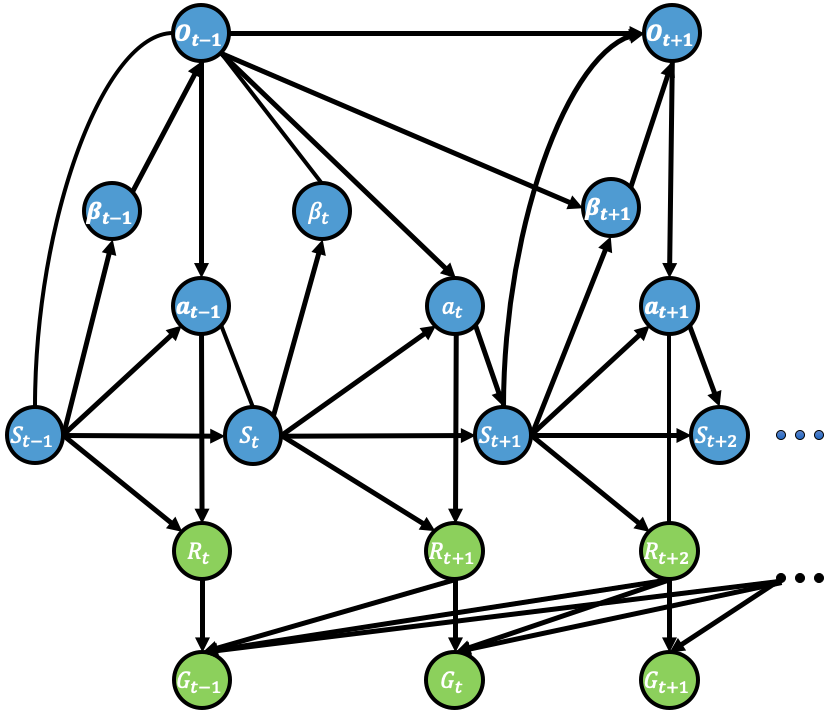
\includegraphics[width=0.5\linewidth]{Part1/figures/oc_smdp.png}\\
  \caption{\label{fig:oc_smdp} An Illustration of the SMDP Option
    Framework. An option $\ro_{t-1}$ is selected by
    master policy $P(\ro_{t-1}|\rvs_{t-1})$ at time step
    $t-1$. At time step $t$, termination function
    $\beta_{o_{t-1}}(\rvs_t)$ determines to continue option
    $\ro_{t-1}$. So that there is no random variable $\ro_t$ at
    time step $t$ compared to there are random variables $\rvo$
    at every time step in MDP formulation
    (figure~\ref{fig:oc_pgm}).}
\end{figure*}
Due to the SMDP formulation, an option can only be improved when
the option terminates. We refer this as the SMDP-style learning
which is sample inefficient and prevents applying SOTA MDP based
algorithms such as the Proximal Policy Optimization (PPO)
algorithm \cite{schulman2017proximal}.



\subsection{HMM dynamics for the Option Framework}
\label{sec:appen_hmm}

We follow \citename{bishop2006pattern}'s formulation of mixture
distribution and Probabilistic Graphical Models (PGMs). By
introducing option variables as latent variables and adding extra
dependencies between them, we show that the conventional SMDP
version of the option framework
\cite{bacon2017option,sutton2018reinforcement,sutton1999between,harb2018waiting,zhang2019dac}
has an MDP equivalence.
\begin{figure*}[th!]
  \centering
  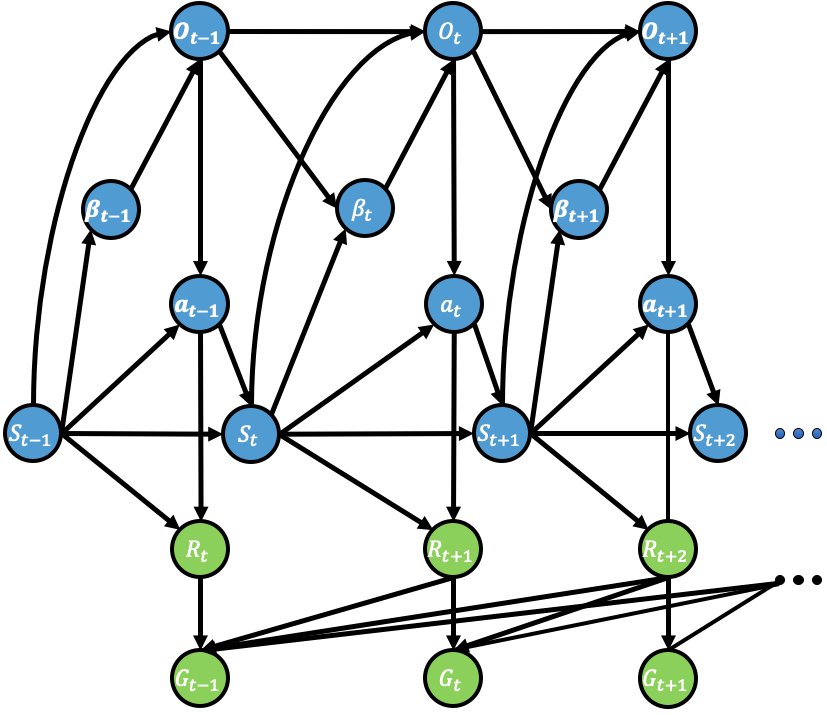
\includegraphics[width=0.5\linewidth]{Part1/figures/oc_pgm.png}\\
  \caption{\label{fig:oc_pgm} PGM of the MDP Option Framework}
\end{figure*}
Following \citet{bishop2006pattern}'s notation, we use bolded
letter $\rvs\in\sS$ to denote a random variable and normal letter
$\rs$ to denote its realization. Without special clarification, a
random vector can have either a vector of continuous or discrete
entries. Vector $\rvo\in\sO$ is an $M$-dimensional one-hot vector
and each entry $\ro\in\{0,1\}$ is a binary random variable.
$P(\rvo_t|\rvs_t)$ denotes the probability distribution over
one-hot vector $\rvo$ at time step $t$ conditioned on state
$\rvs_t$. $P(\rvo_t=\ro_t|\rvs_t)$ denotes a probability entry (a
scalar value) of the random variable $\rvo_t$ with a realization
at time step $t$ where $\ro_t=1$ and $\ro\in\rvo_t/\ro_t=0$.
% todo: define an option set P_o(a) P_o(b) I

In figure~\ref{fig:oc_pgm}, $\rvs\in\sS$, $\rvo\in\sO^M$,
$\rvb\in\sB^M$ and $\rva \in \sA$, denote the state, option,
termination and action random variable respectively. $\rvo$ is an
$M$-dimensional one-hot vector and $\rvb$ is an $M$-dimensional
binary vector where each entry $\rb\in\{0,1\}$. $M$ is the number
of options. $R_{t+1}$ is the actual reward received from the
environment after executing action $\rva_{t}$ in state $\rvs_t$.
$G_t=R_{t+1}+\gamma R_{t+2}+\gamma^2R_{t+3}\cdots$ is the
discounted expected return where $\gamma\in \sR$ is a discount
factor.

The termination policy distribution
$P(\rvb_t|\rvs_t,\rvo_{t-1}):\sS\times\sO\rightarrow\sB$ can be
formulated as a mixture distribution\footnote{Different from
  conventional formulation which only depends on state $\rvs_t$,
  our termination function has an extra dependence on
  $\rvo_{t-1}$} conditioned on option vector (the one-hot vector)
$\rvo_{t-1}$ and state $\rvs_t$.
\begin{equation}
  \label{eq:oc_beta_p}
P(\rvb_t|\rvs_t,\rvo_{t-1}) = \prod_{\ri\in\rvo_{t-1}}P_{\ri}(\rb_t|\rvs_t)^{\ri}.
\end{equation}

Because each option has its own \textbf{termination policy}
$P_o(\rvb|\rvs)$, with a slightly abuse of notation, in
equation~(\ref{eq:oc_beta_p}) we use
$P(\rvb_t|\rvs_t,\rvo_{t-1})$ to denote the termination policy
activated at time step $t$ by previous chosen option
$\rvo_{t-1}$. To keep notation uncluttered, we use
$\beta_t=P(\rvb_t=1|\rvs_t,\rvo_{t-1})$ to denote the probability
of option $\rvo_{t-1}$ terminates at time step $t$ and
$(1-\beta_t) = P(\rvb_t=0|\rvs_t,\rvo_{t-1})$ to denote the
probability of continuation.

Conventionally, master policy \cite{zhang2019dac} (also called
``policy-over-options''~\cite{sutton1999between,bacon2017option}))
is defined as:
\begin{equation}
  \label{eq:oc_master}
  P(\rvo_t|\rvs_t).
\end{equation}
Similarly, we propose a novel \textbf{mixture master policy} as a
mixture distribution\footnote{Different from conventional
  formulation which only depends on state $\rvs_t$, our mixture
  master policy has extra dependencies on $\rvo_{t-1}$ and
  $\rvb_t$}:

\begin{equation}
  \label{eq:oc_po}
P(\rvo_t|\rvs_t, \rvb_t,\rvo_{t-1}) = P(\rvo_t|\rvs_t)^{\rb_t}P(\rvo_t|\rvo_{t-1})^{1-\rb_t},
\end{equation}
~where $P(\rvo_t|\rvo_{t-1})$ is a degenerated probability
distribution~\cite{puterman2014markov}

\begin{equation}
  \label{eq:deg_puterman}
P(\rvo_t|\rvo_{t-1}) = 
\begin{cases}
  1&\;\text{if } \rvo_t=\rvo_{t-1},\\
  0&\;\text{if } \rvo_t\neq\rvo_{t-1}.
\end{cases}
\end{equation}

As shown in equation~(\ref{eq:oc_po}), the master policy only
exists when $\rb_t=1$ the option terminates. Therefore, PPOC
\cite{klissarov2017learnings} uses inaccurate gradients for
updating the master policy during an option's execution.

According to the conditional dependency relationships in PGM
(figure~\ref{fig:oc_pgm}), the joint probability distribution of
$\rvo_t$ and $\rvb_t$ can be written as:
\begin{equation}
  \label{eq:oc_ob_p}
  P(\rvo_t,\rvb_t|\rvs_t,\rvo_{t-1})=P(\rvb_t|\rvs_t,\rvo_{t-1})P(\rvo_t|\rvs_t, \rvb_t,\rvo_{t-1}),
\end{equation}
~and the marginal probability distribution can be written as:
\begin{align}
  \label{eq:oc_oso_p}
  P(\rvo_t|\rvs_t,\rvo_{t-1})&=\sum_{\rvb_t}P(\rvb_t|\rvs_t,\rvo_{t-1})P(\rvo_t|\rvs_t, \rvb_t,\rvo_{t-1})\\
  \nonumber &=P(\rvb_t=0|\rvs_t,\rvo_{t-1})P(\rvo_t|\rvo_{t-1}) +P(\rvb_t=1|\rvs_t,\rvo_{t-1})P(\rvo_t|\rvs_t) \\
\nonumber                             &=(1-\beta_t)P(\rvo_t|\rvo_{t-1}) +\beta_tP(\rvo_t|\rvs_t)\\
  \nonumber&=(1-\beta_t)\1_\mathrm{\rvo_t=\rvo_{t-1}} +\beta_tP(\rvo_t|\rvs_t).
\end{align}

The \textbf{intra-option (action) policy} distribution can also
be formulated as a mixture distribution
\begin{equation}
  \label{eq:oc_a_p}
  P(\rva_t|\rvs_t,\rvo_t) = \prod_{\ri\in\rvo_t}P_{\ri}(\rva_t|\rvs_t)^{\ri}.
\end{equation}
Therefore, the dynamics of the PGM in
figure~\ref{fig:oc_pgm} can be written as:
\begin{align}
  \label{eq:oc_pgm_joint}
\nonumber  P(\tau) = &P(\rvs_0)P(\rvo_0)P(\rva_0|\rvs_0,\rvo_0)\\
  &\prod_{t=1}^\infty P(\rvs_t|\rvs_{t-1},\rva_{t-1})P(\rvb_t|\rvs_t,\rvo_{t-1})P(\rvo_t|\rvb_t,\rvs_t,\rvo_{t-1})P(\rva_{t}|\rvs_{t},\rvo_{t}),
\end{align}
~where
$P(\tau)=P(\rvs_0,\rvo_0,\rva_0,\rvs_1,\rvb_1,\rvo_1,\rva_1,\ldots)$
denotes the joint distribution of the PGM. Notice that under this
formulation, $P(\tau)$ is actually an HMM with $\rvs_t$, $\rva_t$
as observable random variables and $\rvb_t$, $\rvo_t$ as latent
variables.

It is worth to mention that equation~(\ref{eq:deg_puterman}) is
essentially the indicator function
$\1_\mathrm{\rvo_t=\rvo_{t-1}}$ used in conventional SMDP option
framework papers and the last line in
equation~(\ref{eq:oc_oso_p}) is identical to transitional
probability distribution in their formulation. However, as we
show in this section, by adding latent variables $\rvo_{t-1}$ and
introducing the dependency between $\rvo_{t}$ and $\rvb_t$, our
formulation is essentially an HMM. It
% todo: contribution
opens the door to introduce many well developed PGM algorithms
such as message passing~\cite{forney1973viterbi} and variational
inference~\cite{hoffman2013stochastic} to the reinforcement
learning framework. As we show below, the nice conditional
independence relationships enjoyed by this model also enable us
to prove the equivalence between the option framework's SMDP and
MDP formulation.

\subsection{MDP formulation for the Option Framework}
\label{sec:appen_mdp}

With PGM in hand, we now prove that the HMM formulated MDP option
framework has identical value functions with the conventional
SMDP option framework\cite{bacon2017option,sutton1999between}. In
this section, we first show that all value functions defined on
our PGM are identical to the SMDP formulation. We will prove that
the gradients are also the same in next section.

We follow \citename{sutton2018reinforcement}'s notation in this
section and write value functions for MDP below:

\begin{align}
  \label{eq:oc_v}
  \nonumber  V[\rvs_t] &= \E[G_t|\rvs_t] = \sum_{G_t}G_t\sum_{\rvo_t}P(G_t,\rvo_t|\rvs_t)\\
  \nonumber  &= \sum_{\rvo_t}P(\rvo_t|\rvs_t)\sum_{G_t}G_tP(G_t|\rvs_t, \rvo_t)\\
  \nonumber  &= \sum_{\rvo_t}P(\rvo_t|\rvs_t)\E[G_t|\rvo_t, \rvs_t]\\
  &=\sum_{\rvo_t}P(\rvo_t|\rvs_t)Q_{O}[\rvo_t,\rvs_t],
\end{align}
~where $V[\rvs_t]$ is the state value
function\cite{sutton2018reinforcement} and $Q_O[\rvo_t,\rvs_t]$
is the option value
function\cite{bacon2017option,sutton1999between}. Note that in
deriving equation~(\ref{eq:oc_v}) we only use summation rule and
production rule, the conditional dependency relationships in PGM
(figure~\ref{fig:oc_pgm}) are not used. The option value function
$Q_O[\rvo_t,\rvs_t]$ can be further expanded as:
\begin{align}
  \label{eq:oc_qos}
  \nonumber  Q_O[\rvo_t,\rvs_t] &= \E[G_t|\rvo_t, \rvs_t] = \sum_{\rva_t}P(\rva_t|\rvs_t,\rvo_t)\E[G_t|\rvo_t, \rvs_t,\rva_t]\\
&= \sum_{\rva_t}P(\rva_t|\rvs_t,\rvo_t)Q_U[\rvo_t, \rvs_t,\rva_t],
\end{align}
~where $Q_U[\rvo_t, \rvs_t,\rva_t]$ is the option-action value
function.

\begin{prop}
  \label{prop:oc_q_soa}
  MDP formulation has identical state value function $V[\rvs_t]$
  and option value function $Q_O[\rvo_t,\rvs_t]$ to SMDP
  formulations
\end{prop}

\begin{proof}
  Note that in derivations above we only use summation and
  production rules. Both equation~(\ref{eq:oc_v})
  and~(\ref{eq:oc_qos}) are identical to the conventional SMDP
  option framework.
\end{proof}

From now on, we will continue derivations with conditonal
independence relationships encoded in PGM (Chapter 8.2.1
\cite{bishop2006pattern}). Following
\citename{bishop2006pattern}'s notation, we use $A$, $B$ and $C$
to denote three non-overlapping sets of arbitrarily many random
variables. Sets $A$ and $B$ are conditional independent on set
$C$ if $P(A,B|C)=P(A|C)P(B|C)$, denoted as $A\bigCI B \;|\; C$.
We mainly use head-to-tail conditional independence properties
(Chapter 8.2.1 \cite{bishop2006pattern}) in this section. We have
following conditional independence relationships from PGM
(figure~\ref{fig:oc_pgm}):


\begin{align}
\label{eq:c1}  \{R_{t+2},G_{t+1}\}&\bigCI \{\rvb_{t+1}\} &|\;&\{\rvo_{t+1}\},\\
\label{eq:c2} \{R_{t+2},G_{t+1}\}&\bigCI \{\rvs_t\} &|\;&\{\rvs_{t+1},\rvo_t\},\\
\label{eq:c3}  \{R_{t+2},G_{t+1}\}&\bigCI \{\rva_t\} &|\;&\{\rvs_{t+1}\},\\
\label{eq:c4}  \{R_{t+2},G_{t+1}\}&\bigCI \{\rvo_t\} &|\;&\{\rvs_{t+1},\rvo_{t+1}\},\\
\label{eq:c5}  \{R_{t+1},G_{t},\rvs_{t+1}\}&\bigCI \{\rvo_t\} &|\;&\{\rva_{t}\}.
\end{align}

With above conditional independence relationships in hand, we now
show that the MDP formulation has identical value functions to
the conventional SMDP
formulation\cite{sutton1999between,bacon2017option}.

\begin{prop}
  \label{prop:oc_q_soa}
  MDP formulation has identical option-action value function
  $Q_U[\rvo_t, \rvs_t,\rva_t]$ to SMDP formulations
\begin{equation}
  \label{eq:oc_q_soa}
  Q_U[\rvo_t, \rvs_t,\rva_t]=r(\rvs_t,\rva_t)+\gamma\sum_{\rvs_{t+1}}P(\rvs_{t+1}|\rvs_t,\rva_t)U[\rvs_{t+1},\rvo_t].
\end{equation}
\end{prop}

\begin{proof}
\begin{align*}
  Q_U[\rvo_t, \rvs_t,\rva_t] = &\E[G_t|\rvo_t, \rvs_t,\rva_t] &\text{\;} \\
  = &\E[R_{t+1}+\gamma G_{t+1}|\rvo_t, \rvs_t,\rva_t] \\
  =&\E[R_{t+1}|\rvs_t,\rva_t]+\gamma\sum_{G_{t+1}}G_{t+1}\sum_{\rvs_{t+1}}P(\rvs_{t+1}|\rvs_t,\rvo_t,\rva_t)P(G_{t+1}|\rvs_{t+1},\rvo_t,\rvs_t,\rva_t)\\
  =&r(\rvs_t,\rva_t)+\gamma\sum_{G_{t+1}}G_{t+1}\sum_{\rvs_{t+1}}P(\rvs_{t+1}|\rvs_t,\rva_t)P(G_{t+1}|\rvs_{t+1},\rvo_t)\\
  =&r(\rvs_t,\rva_t)+\gamma\sum_{\rvs_{t+1}}P(\rvs_{t+1}|\rvs_t,\rva_t)\E[ G_{t+1}|\rvs_{t+1},\rvo_t ]\\
  =&r(\rvs_t,\rva_t)+\gamma\sum_{\rvs_{t+1}}P(\rvs_{t+1}|\rvs_t,\rva_t)U[\rvs_{t+1},\rvo_t].
\end{align*}
\end{proof}


\begin{prop}
  \label{prop:oc_u}
  MDP formulation has identical option-value function upon
  arrival $U[\rvs_{t+1},\rvo_t]$ to SMDP
  formulations\footnote{Both equations~(\ref{eq:oc_u_qv})
    and~(\ref{eq:oc_u_qa}) is largely used in the conventional
    SMDP papers\cite{sutton1999between,bacon2017option}.}
 \begin{align}
\label{eq:oc_u_qv}  U[\rvs_{t+1},\rvo_t]= &(1-\beta_{t+1})Q_O[\rvo_{t+1}=\ro_t,\rvs_{t+1}] +\beta_{t+1}V[\rvs_{t+1}]\\
 \label{eq:oc_u_qa} = &Q_O[\rvo_{t+1}=\ro_t,\rvs_{t+1}] -\beta_{t+1}A[\rvo_{t+1}=\ro_t,\rvs_{t+1}].
\end{align}
\end{prop}


\begin{proof}
 \begin{align*}
  U[\rvs_{t+1},\rvo_t]=&\E[ G_{t+1}|\rvs_{t+1},\rvo_t ]\\
  =&\sum_{G_{t+1}}G_{t+1}\\
                       &\sum_{\rvo_{t+1}}\sum_{\rvb_{t+1}}P(\rvb_{t+1}|\rvo_t,\rvs_{t+1})P(\rvo_{t+1}|\rvb_{t+1},\rvo_t,\rvs_{t+1})P(G_{t+1}|\rvo_{t+1},\rvb_{t+1},\rvo_t,\rvs_{t+1})\\
  =&\sum_{\rvo_{t+1}}\sum_{\rvb_{t+1}}P(\rvb_{t+1}|\rvo_t,\rvs_{t+1})P(\rvo_{t+1}|\rvb_{t+1},\rvo_t,\rvs_{t+1})\sum_{G_{t+1}}G_{t+1}P(G_{t+1}|\rvo_{t+1},\rvs_{t+1})\\
  = &\sum_{\rvo_{t+1}}\big[(1-\beta_{t+1})\1_\mathrm{\rvo_{t+1}=\rvo_t} +\beta_{t+1}P(\rvo_{t+1}|\rvs_{t+1})\big]Q_O[\rvo_{t+1},\rvs_{t+1}]\\
  = &(1-\beta_{t+1})Q_O[\rvo_{t+1}=\ro_t,\rvs_{t+1}] +\beta_{t+1}V[\rvs_{t+1}]\\
  = &Q_O[\rvo_{t+1}=\ro_t,\rvs_{t+1}] -\beta_{t+1}A[\rvo_{t+1}=\ro_t,\rvs_{t+1}].
\end{align*}
~from line 3 to line 4 use equation (\ref{eq:c1}) and
(\ref{eq:c4}). From line 4 to line 5 use equation
(\ref{eq:oc_oso_p}) and definition of $Q_O$. The second last line
use equation~(\ref{eq:oc_v}). The last line use the definition of
advantage function $A$.
\end{proof}

Under our MDP formulation, we also propose proposition
\ref{approp:oc_u_pgm}. We derive our gradient theorems based on
equation~(\ref{eq:oc_u_pgm}) in section~\ref{sec:appen_mdp_grad}.
This important relationship largely simplify derivations than the
original paper~\cite{bacon2017option} as well as give rise to the
SA.

\begin{prop}
    \label{approp:oc_u_pgm}
    The option-value function upon arrival $U[\rvs_{t+1},\rvo_t]$
    is an expectation over option value function
    $Q_O[\rvo_{t+1},\rvs_{t+1}]$ conditioned on previous option
    $O_{t}$
  \begin{equation}
    \label{eq:oc_u_pgm}
    U[\rvs_{t+1},\rvo_t]= \sum_{\rvo_{t+1}}P(\rvo_{t+1}|\rvo_t,\rvs_{t+1})Q_O[\rvo_{t+1},\rvs_{t+1}].
  \end{equation}
\end{prop}

\begin{proof}
  Following proof of proposition \ref{prop:oc_u},
 \begin{align*}
  \nonumber U[\rvs_{t+1},\rvo_t]=&\sum_{\rvo_{t+1}}\sum_{\rvb_{t+1}}P(\rvb_{t+1}|\rvo_t,\rvs_{t+1})P(\rvo_{t+1}|\rvb_{t+1},\rvo_t,\rvs_{t+1})\sum_{G_{t+1}}G_{t+1}P(G_{t+1}|\rvo_{t+1},\rvs_{t+1})\\
=&\sum_{\rvo_{t+1}}P(\rvo_{t+1}|\rvo_t,\rvs_{t+1})Q_O[\rvo_{t+1},\rvs_{t+1}].
\end{align*}
\end{proof}

\subsection{Gradients for the MDP Option Framework}
\label{sec:appen_mdp_grad}

In above sections, we formulate dynamics of the option framework
using HMM and prove the MDP build on it has identical value
functions to SMDP formulation. In this section we will prove that
both MDP and SMDP formulations~\cite{bacon2017option} share same
intra-option and termination gradients. Our derivations is
largely simplified by equation~(\ref{eq:oc_u_pgm}) compared to
previous work.

Let $\theta_a$ denote parameter vector for intra-option policies
$P(\rva_t|\rvs_t,\rvo_t;\theta_a)$ and $\theta_b$ denote
parameter vector for termination policies
$P(\rvb_t|\rvs_t,\rvo_{t-1};\theta_b)$. To keep notation
uncluttered, we drop the dependency on parameter vector $\theta$
in derivations below.

\begin{prop}
  \label{approp:oc_a_grad}
  MDP formulation has identical Intra-Option Policy Gradient with
  SMDP formulation in~\cite{bacon2017option}.
  \begin{align}
    \nonumber    \frac{\partial Q_O[ \rvs_t,\rvo_t ]}{\partial \theta_a}=
    \sum_{\rk=0}^\infty&\sum_{\rvs_{t+k},\rvo_{t+k}}P_\gamma^{(k)}(\rvs_{t+k},\rvo_{t+k}|\rvs_t,\rvo_t)\\
    \label{eq:oc_a_grad}    &\sum_{\rva_{t+k}}\frac{\partial P(\rva_{t+k}|\rvs_{t+k},\rvo_{t+k})}{\partial \theta_a}Q_U(\rvs_{t+k},\rvo_{t+k},\rva_{t+k}).
  \end{align}
\end{prop}

\begin{proof}
  This is a direct result by taking gradient of $\theta_a$ with
  respect to equation~(\ref{eq:oc_qos}) by using
  equation~(\ref{eq:oc_q_soa}) and (\ref{eq:oc_u_pgm}):
\begin{align*}
  \frac{\partial Q_O[ \rvs_t,\rvo_t ]}{\partial \theta_a}=&\sum_{\rva_t}\frac{\partial P(\rva_t|\rvs_t,\rvo_t)}{\partial \theta_a}Q_U[\rvo_t, \rvs_t,\rva_t]+\gamma\sum_{\rva_t}P(\rva_t|\rvs_t,\rvo_t)\frac{\partial Q_U[\rvo_t, \rvs_t,\rva_t]}{\partial \theta_a}\\
  =&\sum_{\rva_t}\frac{\partial P(\rva_t|\rvs_t,\rvo_t)}{\partial \theta_a}Q_U[\rvo_t, \rvs_t,\rva_t]\\
                                                        &+ \gamma\sum_{\rva_t}P(\rva_t|\rvs_t,\rvo_t)\sum_{\rvs_{t+1}}P(\rvs_{t+1}|\rvs_t,\rva_t)\frac{\partial U[\rvo_t,\rvs_{t+1}]}{\partial \theta_a}\\
  =&\sum_{\rva_t}\frac{\partial P(\rva_t|\rvs_t,\rvo_t)}{\partial \theta_a}Q_U[\rvo_t, \rvs_t,\rva_t]\\
                                                        &+ \gamma\sum_{\rvs_{t+1}}P(\rvs_{t+1}|\rvs_t,\rvo_t)\sum_{\rvo_{t+1}}P(\rvo_{t+1}|\rvs_{t+1},\rvo_t)\frac{\partial Q_O[\rvo_{t+1},\rvs_{t+1}]}{\partial \theta_a}\\
  =&\sum_{\rva_t}\frac{\partial P(\rva_t|\rvs_t,\rvo_t)}{\partial \theta_a}Q_U[\rvo_t, \rvs_t,\rva_t] + \gamma\sum_{\rvo_{t+1},\rvs_{t+1}}P(\rvs_{t+1},\rvo_{t+1}|\rvs_{t},\rvo_t)\frac{\partial Q_O[\rvo_{t+1},\rvs_{t+1}]}{\partial \theta_a}\\
  =&\sum_{\rk=0}^\infty\sum_{\rvs_{t+k},\rvo_{t+k}}P_\gamma^{(k)}(\rvs_{t+k},\rvo_{t+k}|\rvs_t,\rvo_t)\\
                                                        &\sum_{\rva_{t+k}}\frac{\partial P(\rva_{t+k}|\rvs_{t+k},\rvo_{t+k})}{\partial \theta_a}Q_U(\rvs_{t+k},\rvo_{t+k},\rva_{t+k}).
\end{align*}
\end{proof}

\begin{prop}
  \label{approp:oc_b_grad}
  MDP formulation has identical Termination Policy Gradient with
  SMDP formulation in~\cite{bacon2017option}.
  \begin{align}
    \label{eq:oc_b_grad}   \frac{\partial U[ \rvs_{t+1},\rvo_t ]}{\partial \theta_b}=
    -\sum_{\rk=0}^\infty&\sum_{\rvs_{t+1+k},\rvo_{t+k}}P_\gamma^{(k)}(\rvs_{t+1+k},\rvo_{t+k}|\rvs_{t+1},\rvo_t)
                         \frac{\partial \beta_{t+1+k}}{\partial \theta_b}A[ \rvs_{t+k+1},\rvo_{t+k+1}=\rvo_{t+k}].
  \end{align}
\end{prop}

\begin{proof}
  We first show the gradient of $\theta_b$ with respect to
  equation~(\ref{eq:oc_oso_p}) and (\ref{eq:oc_qos}) separately:

  \begin{align}
    \label{eq:oc_oso_p_grad} \frac{\partial P(\rvo_{t+1}|\rvs_{t+1},\rvo_{t})}{\partial \theta_b} = &\big[P(\rvo_{t+1}|\rvs_{t+1})-\1_\mathrm{\rvo_t=\rvo_{t-1}}\big]\frac{\partial \beta_{t+1}}{\partial \theta_b}\\
    \nonumber\frac{\partial Q_O[\rvo_{t+1},\rvs_{t+1}]}{\partial \theta_b} =& \sum_{\rva_{t+1}}P(\rva_{t+1}|\rvs_{t+1},\rvo_{t+1})\sum_{\rvs_{t+2}}P(\rvs_{t+2}|\rvs_{t+1},\rva_{t+1})\frac{\partial U[\rvs_{t+2},\rvo_{t+1}]}{\partial \theta_b}\\
 \label{eq:oc_qos_grad}   =&\sum_{\rvs_{t+2}}P(\rvs_{t+2}|\rvs_{t+1},\rvo_{t+1})\frac{\partial U[\rvs_{t+2},\rvo_{t+1}]}{\partial \theta_b}.
  \end{align}

  The equation~(\ref{eq:oc_b_grad}) is a direct result by taking
  gradient of $\theta_b$ with respect to
  equation~(\ref{eq:oc_u_pgm}) and using above results:
  \begin{align*}
    \frac{\partial U[ \rvs_{t+1},\rvo_t ]}{\partial \theta_b}=&\sum_{\rvo_{t+1}}\frac{\partial P(\rvo_{t+1}|\rvo_t,\rvs_{t+1})}{\partial \theta_b}Q_O[\rvo_{t+1},\rvs_{t+1}] + \sum_{\rvo_{t+1}}P(\rvo_{t+1}|\rvo_t,\rvs_{t+1})\frac{\partial Q_O[\rvo_{t+1},\rvs_{t+1}]}{\partial \theta_b}\\
    =&\sum_{\rvo_{t+1}} \big[P(\rvo_{t+1}|\rvs_{t+1})-\1_\mathrm{\rvo_t=\rvo_{t-1}}\big]Q_O[\rvo_{t+1},\rvs_{t+1}]\frac{\partial \beta_{t+1}}{\partial \theta_b}\\
    &+\sum_{\rvo_{t+1}}P(\rvo_{t+1}|\rvo_t,\rvs_{t+1})\gamma\sum_{\rvs_{t+2}}P(\rvs_{t+2}|\rvs_{t+1},\rvo_{t+1})\frac{\partial U[\rvs_{t+2},\rvo_{t+1}]}{\partial \theta_b}\\
    =& \big[V[ \rvs_{t+1} ]-Q_O[\rvo_{t+1}=\rvo_t,\rvs_{t+1}]\big]\frac{\partial \beta_{t+1}}{\partial \theta_b}\\
    &+\gamma\sum_{\rvo_{t+1},\rvs_{t+2}}P(\rvs_{t+2},\rvo_{t+1}|\rvs_{t+1},\rvo_{t})\frac{\partial U[\rvs_{t+2},\rvo_{t+1}]}{\partial \theta_b}\\
    =& -A[\rvo_{t+1}=\rvo_t,\rvs_{t+1}]\frac{\partial \beta_{t+1}}{\partial \theta_b}+\gamma\sum_{\rvo_{t+1},\rvs_{t+2}}P(\rvs_{t+2},\rvo_{t+1}|\rvs_{t+1},\rvo_{t})\frac{\partial U[\rvs_{t+2},\rvo_{t+1}]}{\partial \theta_b}\\
    =&-\sum_{\rk=0}^\infty\sum_{\rvs_{t+1+k},\rvo_{t+k}}P_\gamma^{(k)}(\rvs_{t+1+k},\rvo_{t+k}|\rvs_{t+1},\rvo_t)
                         \frac{\partial \beta_{t+1+k}}{\partial \theta_b}A[ \rvs_{t+k+1},\rvo_{t+k+1}=\rvo_{t+k}].
  \end{align*}
  
\end{proof}

\subsection{Summary}
\label{sec:equiva_conc}
In this previous sections, we prove that an MDP equivalence to
the SMDP. Briefly, we propose a novel MDP ``mixture master
policy'' (\Secref{sec:appen_hmm}). Unlike the conventional SMDP
master policy that only depends on the current state, the mixture
master policy has extra dependencies on the termination function
and the previously activated option. We then prove that the MDP
has identical optimal properties with the SMDP option framework
\cite{sutton1999between} and identical policy gradients with the
option-critic architecture \cite{bacon2017option}. We summarize
our results as the following theorem:

\begin{thm}
  \label{theo:smdp_mdp}
  The SMDP formulated option framework, which employs Markovian
  options, has an underlying MDP equivalence.
\end{thm}
\begin{prop}
  \label{prop:opt}
  The MDP formulation has identical optimality (value functions)
  with the SMDP option framework~\cite{sutton1999between}.
\end{prop}
\begin{prop}
  \label{prop:pg}
  The MDP formulation has identical policy gradients with the
  option-critic architecture~\cite{bacon2017option}.
\end{prop}

\section{The Skill-Action Architecture}
\label{sec:sa}

In this section, we propose a simple
MDP~\cite{puterman2014markov} implementation of the option
framework: the Skill-Action (SA) architecture. Although the
mixture master policy (Eq.~\ref{eq:oc_po}) is MDP formulated, the
master policy's (Eq.~\ref{eq:oc_master}) gradients are
still blocked by its dependency on the termination function. To
overcome this, we present a marginalized derivation of the
equivalence: the Skill-Action (SA) architecture. SA marginalizes
the termination function away and models the marginalized policy
(Eq.~\ref{eq:oc_oso_p}) directly with a ``skill policy''
(Eq.~\ref{eq:sa_o_p}), which is used to replace both the master
policy and termination function while implements their
functionalities with the attention
mechanism~\cite{vaswani2017attention}. Section~\ref{sec:sa_PGM}
describes the dynamics (Markov process) of SA.
Section~\ref{sec:sa_mdp} defines value functions on top of the
dynamics, thus formulating the MDP. Policy gradient theorems are
then derived. Section~\ref{sec:net_arch} implements SA by
employing neural networks and the Multi-Head Attention
mechanism~\cite{vaswani2017attention}, which enables SA to
temporally extend skills in the absence of the termination
function.


\subsection{Dynamics of the Skill-Action Architecture}
\label{sec:sa_PGM}

\begin{figure*}[thb]
  \centering
  \begin{tabular}{cc}
    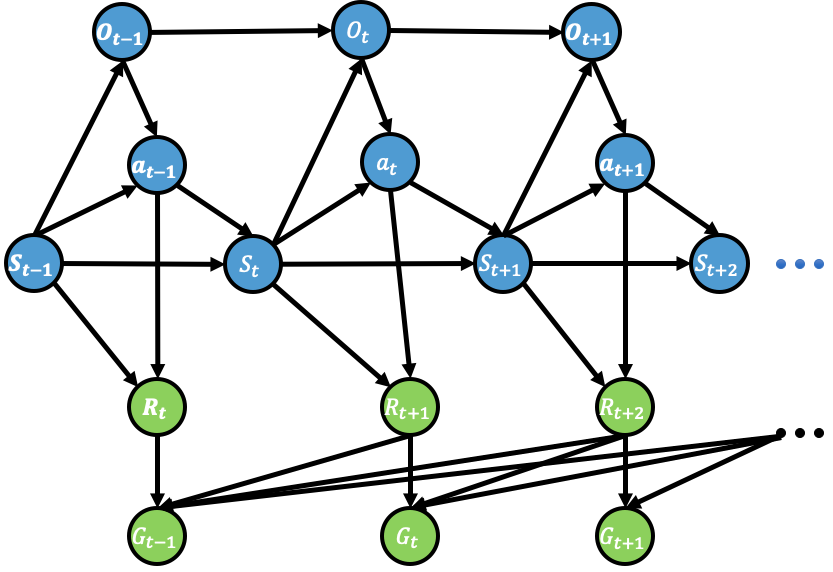
\includegraphics[width=0.45\linewidth]{./Part1/figures/doe.png}&
                                                              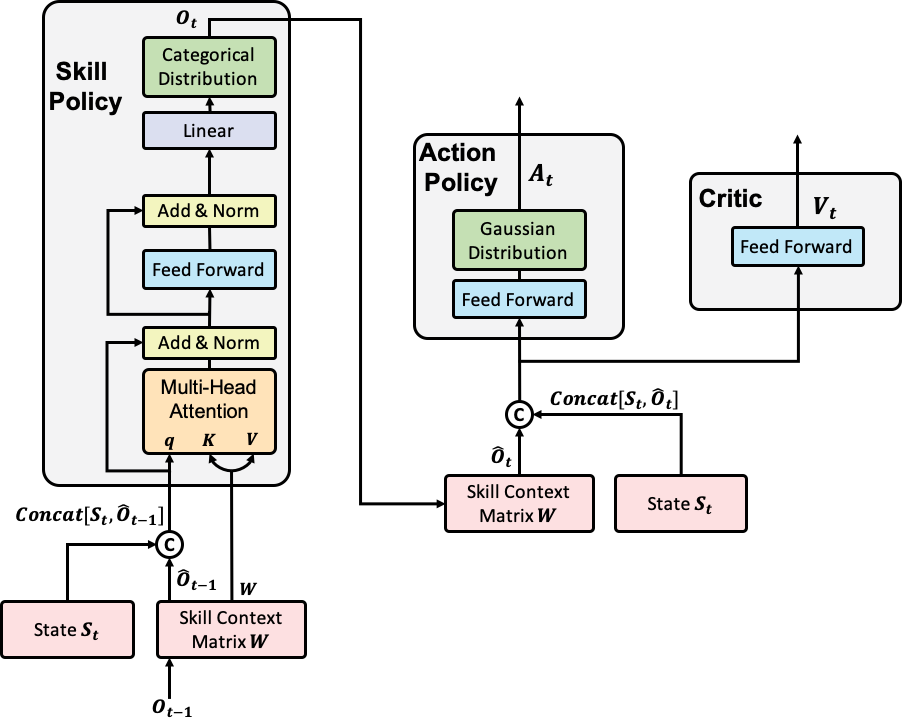
\includegraphics[width=0.45\linewidth]{./Part1/figures/sa_attn_net.png}\\
    {\small (a) PGM of SA}&
                            {\small (b) Network
                            Architecture of SA}\\
   
  \end{tabular}
  \caption{\label{fig:sa_net} The Skill-Action (SA) Architecture}
\end{figure*}

In this section, we define the dynamics (Markov process) of SA.
We first introduce MDP notations. A Markov decision process
$M=\{\sS,\sA,r,P,\gamma\}$ consists of a state space $\sS$, an
action space $\sA$, a state transition function
$P(\rvs_{t+1}|\rvs_t): \sS\rightarrow\sS$, a reward function
$r(\rvs,\rva):\sS\times\sA\rightarrow\sR$, and a discount factor
$\gamma\in\sR$. A policy $\pi=P(\rva|\rvs):\sS\rightarrow \sA$ is
a probability distribution defined over actions conditioning on
states. An expected discounted return is defined as $G_t =
\sum_k^N\gamma^kR_{t+k+1}$, where $R\in\sR$ is the actual reward
received from the environment. The value function
$V[\rvs_t]=\E_{\pi}[G_t|\rvs_t]$ is the expected return starting
at state $\rvs_t$ and following policy $\pi$ thereafter. The
action-value function is defined as $Q[\rvs_t,\rva_t]=
\E_{\tau_\pi}[G_t|\rvs_t,\rva_t]$. An Markov decision process
together with value functions defined on it are referred to as an
MDP~\cite{puterman2014markov}.

Having defined notations of MDP, we propose the dynamics of SA.
Specifically, a \textbf{skill index vector} $\rvo\in\sZ^M_2$ is
an $M$-dimensional one-hot vector, where $M$ denotes the total
number of skills to learn. Each entry $\ro\in\{0,1\}$ is a binary
random variable. $\ro_i=1$ means that the $i$-th skill is
activated. A \textbf{skill context matrix}
\cite{kosiorek2019stacked} $\mW_S\in \sR^{M\times E}$ is a
learnable parameter containing $M$ rows of $E$ dimensional real
vectors, the $i$-th row of $\mW_S$ corresponds to the $i$-th
skill $\ro_i$, and different columns encode different properties
of a skill. A \textbf{skill context vector} $\hat{\rvo}_t$ is
defined as:
\begin{equation}
  \label{eq:sa_skill_vector}
  \hat{\rvo}_t=\mW_S^{T}\cdot\rvo_t, \;\hat{\rvo}_t\in \sR^{E}.
\end{equation}
The \textbf{skill policy} is defined as:
\begin{equation}
  \label{eq:sa_o_p}
  P(\hat{\rvo}_t|\rvs_t,\hat{\rvo}_{t-1};\mW_s): \sS\times\sR^{E} \rightarrow \sR^{E},
\end{equation}
% todo: explain the functionality of P(o); what's the motivation;
% how is it implemented; advantages; contributions
which is a probability distribution over skill context vector
$\hat{\rvo}_{t}$ conditioned on state $\rvs_t$ and previous
sampled skill context vector $\hat{\rvo}_{t-1}$, with $\mW_S$ as
its learnable parameters.

The \textbf{action policy} is defined as:
\begin{equation}
  \label{eq:sa_a_p}
  P(\rva_t|\rvs_t,\hat{\rvo}_t): \sS\times\sR^E\rightarrow\sA,
\end{equation}
which is a probability distribution over the action random
variable $\rva_t\in\sA$ conditioned on the skill context vector
$\hat{\rvo}_t$ and state $\rvs_t$, and decodes them into primary
actions.

With both skill and action policies in hand, the dynamics of the
SA are defined as a Probabilistic Graphical Model
(PGM)~\cite{koller2009probabilistic} (Figure~\ref{fig:sa_net}
(a)):
\begin{align}
  \label{eq:sa_pgm_joint}
  \nonumber  P(\tau) = &P(\rvs_0)P(\hat{\rvo}_0)P(\rva_0|\rvs_0,\hat{\rvo}_0)\\
                       &\prod_{t=1}^\infty P(\rvs_t|\rvs_{t-1},\rva_{t-1})P(\hat{\rvo}_t|\rvs_t,\hat{\rvo}_{t-1})P(\rva_{t}|\rvs_{t},\hat{\rvo}_{t}),
\end{align}
where
$P(\tau)=P(\rvs_0,\hat{\rvo}_0,\rva_0,\rvs_1,\hat{\rvo}_1,\rva_1,\ldots)$
denotes the joint distribution of the PGM. Note that under this
formulation, $P(\tau)$ is actually an Hidden Markov Model (HMM)
with $\rvs_t$, $\rva_t$ as observable random variables and
$\hat{\rvo}_t$ as latent variables.

\subsection{MDP of the Skill-Action Architecture}
\label{sec:sa_mdp}

With SA's dynamics in hand, in this section, we first propose a
novel ``skill value upon arrival function'' and theoretically
prove that it has a smaller variance than the conventional value
function. This property is empirically justified in
Section~\ref{sec:exp_perf} and further discussed in
\Secref{sec:append_gist}. Then, we derive the recursive
formulation of value functions and formulate the MDP. Based on
the MDP, skill and action policies' gradients theorems are
finally derived.

Rather than use the conventional value function $V[\rvs_t]$, we
define the \textbf{skill value upon arrival function}
$V[\rvs_t,\hat{\rvo}_{t-1}]$ as:
\begin{equation}
  \label{eq:sa_v}
  V[\rvs_t,\hat{\rvo}_{t-1}]=\E[G_t|\rvs_t,\hat{\rvo}_{t-1}]= \sum_{\hat{\rvo}_t}P(\hat{\rvo}_t|\rvs_t,\hat{\rvo}_{t-1})Q_O[ \rvs_t,\hat{\rvo}_t].
\end{equation}

\begin{proof}
  Derivations of Eq.~(\ref{eq:sa_v}):
%
\begin{align*}
  V[\rvs_t,\hat{\rvo}_{t-1}]=&\E[G_t|\rvs_t,\hat{\rvo}_{t-1}]\\
  =& \sum_{\hat{\rvo}_t}P(\hat{\rvo}_t|\rvs_t,\hat{\rvo}_{t-1})\E(G_t|\rvs_t,\hat{\rvo}_t,\hat{\rvo}_{t-1})\\
  =& \sum_{\hat{\rvo}_t}P(\hat{\rvo}_t|\rvs_t,\hat{\rvo}_{t-1})\E[ G_t|\rvs_t,\hat{\rvo}_t ]\\
  =& \sum_{\hat{\rvo}_t}P(\hat{\rvo}_t|\rvs_t,\hat{\rvo}_{t-1})Q_O[ \hat{\rvo}_t,\rvs_t],
\end{align*}
%
where from line 2 to line 3 we use the conditional independence
property in PGM that
$G_t\bigCI\hat{\rvo}_{t-1}|\{\rvs_t,\hat{\rvo}_t\}$.
\end{proof}

\begin{prop}
  \label{prop:var_unb}
  $V[ \rvs_t,\hat{\rvo}_{t-1} ]$ is an unbiased estimation of $V[ \rvs_t ]$.
\end{prop}
\begin{proof}
  By law of total expectation:
  $$\E_{\hat{\rvo}_{t-1}}[V[\rvs_t,\hat{\rvo}_{t-1}]]=\E_{\hat{\rvo}_{t-1}}[\E[G_t|\rvs_t,\hat{\rvo}_{t-1}]]=\E[G_t|\rvs_t] = V[\rvs_t]$$
%
thus $V[\rvs_t,\hat{\rvo}_{t-1}]$ is an unbiased estimator of $V[\rvs_t]$.
\end{proof}

\begin{prop}
  \label{prop:var_red}
  The variance of $V[ \rvs_t,\hat{\rvo}_{t-1} ]$ is less than or equal to $V[ \rvs_t ]$.
\end{prop}
\begin{proof}
  By law of total conditional variance:
\begin{align*}
  \text{Var}(V[\rvs_t]) &= \text{Var}([\E[G_t|\rvs_t]]) =\E[\text{Var}(\E[G_t|\rvs_t,\hat{\rvo}_{t-1}])|\rvs_t]+\text{Var}(\E[\E[G_t|\rvs_t,\hat{\rvo}_{t-1}]]|\rvs_t)\\
                        &= \E[\text{Var}(V[\rvs_t,\hat{\rvo}_{t-1}])|\rvs_t]+\text{Var}(\E[V[\rvs_t,\hat{\rvo}_{t-1}]]|\rvs_t)\\
  &\geq \text{Var}(\E[V[\rvs_t,\hat{\rvo}_{t-1}]]|\rvs_t).
\end{align*}
\end{proof}

Eq.~(\ref{eq:sa_v}) states that the skill value function upon
arrival is an expectation over skill value function
$Q_O[\rvs_t,\hat{\rvo}_{t}]$ conditioned on previous skill
$\hat{\rvo}_{t-1}$. The \textbf{skill value function}
$Q_O[\rvs_t,\hat{\rvo}_{t}]$ is defined as:
\begin{align}
  Q_O[\rvs_t,\hat{\rvo}_{t}]=\E[G_t|\rvs_t,\hat{\rvo}_{t}]
  \label{eq:sa_q_o}=\sum_{\rva_t}P(\rva_t|\rvs_t,\hat{\rvo}_{t})Q_A[ \rvs_t,\hat{\rvo}_t,\rva_t],
\end{align}
and the \textbf{skill-action value function} $Q_A[
\rvs_t,\hat{\rvo}_t,\rva_t]$ is defined as:
\begin{align}
\label{eq:sa_q_a}
Q_A[ \rvs_t,\hat{\rvo}_t,\rva_t]&=\E[G_t| \rvs_t,\hat{\rvo}_t,\rva_t]\nonumber\\
   &= r(s,a) + \gamma\sum_{\rvs_{t+1}}P(\rvs_{t+1}|\rvs_t,\rva_t)V[\rvs_{t+1},\hat{\rvo}_t],
\end{align}
%
where $\gamma \in \sR$ is a discounting factor.
\begin{proof}
  \begin{align*}
  Q_A[ \rvs_t,\hat{\rvo}_t,\rva_t]=&\E[G_t| \rvs_t,\hat{\rvo}_t,\rva_t]
                               =\E[R_{t+1}+\gamma G_{t+1}| \rvs_t,\hat{\rvo}_t,\rva_t]\\
  =& r(s,o,a) + \gamma\sum_{\rvs_{t+1}}P(\rvs_{t+1}|\rvs_t,\hat{\rvo}_t,\rva_t)\E[G_{t+1}|\rvs_{t+1},\rvs_t,\hat{\rvo}_t,\rva_t]\\
  =& r(s,a) + \gamma\sum_{\rvs_{t+1}}P(\rvs_{t+1}|\rvs_t,\rva_t)\E[G_{t+1}|\rvs_{t+1},\hat{\rvo}_t]\\
  =& r(s,a) + \gamma\sum_{\rvs_{t+1}}P(\rvs_{t+1}|\rvs_t,\rva_t)V[\rvs_{t+1},\hat{\rvo}_t],
\end{align*}
%
where from line 2 to line 3 we use the conditional independence
property in PGM that $R_{t+1}\bigCI\hat{\rvo}_{t}|\rva_t$,
$G_{t+1}\bigCI\rvs_{t}|\{\rvs_{t+1},\hat{\rvo}_t\}$ and
$G_{t+1}\bigCI\rva_{t}|\rvs_{t+1}$. $\gamma \in \sR$ is a
discounting factor.
\end{proof}

Expanding (Eq.~\ref{eq:sa_q_a}) with (Eq.~\ref{eq:sa_v}) gives us
a recursion formulation from which Bellman equations and policy
gradient theorems are derived. To keep notations uncluttered, we
use $\theta_o$ to denote skill policy's parameters
(Eq.~\ref{eq:sa_o_p}) and $\theta_a$ to denote action policy's
parameters (Eq.~\ref{eq:sa_a_p}). The skill and action policies'
gradient theorems are:
\begin{thm}
  \textbf{ Skill Policy Gradient Theorem: } Given a stochastic skill policy
  differentiable in its parameter vector $\theta_o$, the gradient
  of the expected discounted return with respect to $\theta_o$ is:
  \begin{equation}
    \label{eq:sa_o_grad}
    \frac{\partial V[\rvs_t,\hat{\rvo}_{t-1}]}{\partial \theta_o}=\E[\;\frac{\partial P(\hat{\rvo}'|\rvs',\hat{\rvo})}{\partial \theta_o}Q_O[\rvs',\hat{\rvo}']\;|\;\rvs_t,\hat{\rvo}_{t-1}],
  \end{equation}
  ~where $\hat{\rvo}'$ is one time step later than $\hat{\rvo}$.

  \begin{proof}
    \begin{align*}
      \frac{\partial Q_O[\rvs_t,\hat{\rvo}_t]}{ \partial \theta_o }=& \sum_{\rva_t}P(\rva_t|\rvs_t,\hat{\rvo}_t)\big[r(s,a) + \gamma\sum_{\rvs_{t+1}}P(\rvs_{t+1}|\rvs_t,\rva_t)\frac{\partial V[\rvs_{t+1},\hat{\rvo}_t]}{\partial \theta_o}\big]\\
      =&\sum_{\rvs_{t+1}}\gamma P(\rvs_{t+1}|\rvs_t,\hat{\rvo}_t)\frac{\partial V[\rvs_{t+1},\hat{\rvo}_t]}{\partial \theta_o}\\
      \frac{\partial V[\rvs_t,\hat{\rvo}_{t-1}]}{\partial \theta_o}=&\sum_{\hat{\rvo}_t}\frac{\partial P(\hat{\rvo}_t|\rvs_t,\hat{\rvo}_{t-1})}{\partial \theta_o}Q_O[\rvs_t,\hat{\rvo}_t]+\gamma\sum_{\hat{\rvo}_t}P(\hat{\rvo}_t|\rvs_t,\hat{\rvo}_{t-1})\frac{Q_O[\rvs_t,\hat{\rvo}_t]}{\partial \theta_o}\\
      =&\sum_{\hat{\rvo}_t}\frac{\partial P(\hat{\rvo}_t|\rvs_t,\hat{\rvo}_{t-1})}{\partial \theta_o}Q_O[\rvs_t,\hat{\rvo}_t]
         +\gamma\sum_{\rvs_{t+1},\hat{\rvo}_t}P(\rvs_{t+1},\hat{\rvo}_t|\rvs_t,\hat{\rvo}_{t-1})\frac{\partial V[\rvs_{t+1},\hat{\rvo}_t]}{\partial \theta_o}\\
      =&-\sum_{\rk=0}^\infty\sum_{\rvs_{t+k},\hat{\rvo}_{t+k-1}}\\
                                                              &P_{\gamma}^{(k)}(\rvs_{t+k},\hat{\rvo}_{t+k-1}|\rvs_{t},\hat{\rvo}_{t-1})\sum_{\hat{\rvo}_{t+k}}\frac{\partial P(\hat{\rvo}_{t+k}|\rvs_{t+k},\hat{\rvo}_{t+k-1})}{\partial \theta_o}Q_O[ \rvs_{t+k},\hat{\rvo}_{t+k}]\\
      =&\E[\;\frac{\partial P(\rvo'|\rvs',\rvo)}{\partial \theta_o}Q_O[\rvs',\rvo']\;|\;\rvs_t,\hat{\rvo}_{t-1}].
  \end{align*}
\end{proof}
\end{thm}


\begin{thm}
  \textbf{ Action Policy Gradient Theorem: } Given a stochastic action policy
  differentiable in its parameter vector $\theta_a$, the gradient
  of the expected discounted return with respect to $\theta_a$ is:
  \begin{equation}
    \label{eq:sa_a_grad}
      \frac{\partial Q_O[\rvs_t,\hat{\rvo}_t]}{ \partial \theta_a }=\E[\;\frac{\partial P(\rva|\rvs,\hat{\rvo})}{\partial \theta_a}Q_A[ \rvs,\hat{\rvo},\rva]\; | \; \rvs_t,\hat{\rvo}_t].
  \end{equation}
\begin{proof} Similar to the first equation above, continue expanding
  gradients of $\frac{\partial Q_O}{\partial \theta_a}$ by
  equations~(\ref{eq:sa_v})~(\ref{eq:sa_q_o}) and
  (\ref{eq:sa_q_a}):
    \begin{align*}
      \frac{\partial Q_O[\rvs_t,\hat{\rvo}_t]}{ \partial \theta_a }=&\sum_{\rva_t}\frac{\partial P(\rva_t|\rvs_t,\hat{\rvo}_t)}{\partial \theta_a}Q_A[\rvs_t, \hat{\rvo}_t,\rva_t]+\gamma\sum_{\rvs_{t+1}}P(\rvs_{t+1}|\rvs_t,\hat{\rvo}_t)\frac{\partial V[\rvs_{t+1},\hat{\rvo}_t]}{\partial \theta_a}\\
      =&\sum_{\rva_t}\frac{\partial P(\rva_t|\rvs_t,\hat{\rvo}_t)}{\partial \theta_a}Q_A[\rvs_t, \hat{\rvo}_t,\rva_t]+\gamma\sum_{\rvs_{t+1},\hat{\rvo}_{t+1}}P(\rvs_{t+1},\hat{\rvo}_{t+1}|\rvs_t,\hat{\rvo}_t)\frac{\partial Q_O[\rvs_{t+1},\hat{\rvo}_{t+1}]}{\partial \theta_a}\\
      =&-\sum_{\rk=0}^\infty\sum_{\rvs_{t+k},\hat{\rvo}_{t+k}}\\
      &P_{\gamma}^{(k)}(\rvs_{t+k},\hat{\rvo}_{t+k}|\rvs_{t},\hat{\rvo}_{t})\sum_{\rva_{t+k}}\frac{\partial P(\rva_{t+k}|\rvs_{t+k},\hat{\rvo}_{t+k})}{\partial \theta_a}Q_A[ \rvs_{t+k},\hat{\rvo}_{t+k},\rva_{t+k}]\\
      =&\E[\;\frac{\partial P(\rva_{t+k}|\rvs_{t+k},\hat{\rvo}_{t+k})}{\partial \theta_a}Q_A[ \rvs_{t+k},\hat{\rvo}_{t+k},\rva_{t+k}]\; | \; \rvs_t,\hat{\rvo}_t].
  \end{align*}
\end{proof}
\end{thm}


% towrite:
%As conventional option frameworks, the action policy can also be
%composed of $M$ action policies, in which case all of our
%theorems still hold. However, 

Compared to MDP formulated algorithms, SMDP option frameworks are
sample inefficient and notoriously unstable to
hyperparameters~\cite{zhang2019dac}. The skill and action
policies' gradient theorems enable SA to be compatible with both
MDP on-policy and off-policy algorithms, and thus has much better
stability and convergence. This work is focused on deriving MDPs
of SA and its policy gradient theorems. To be comparable with
previous work \cite{zhang2019dac}, in this paper we directly
apply PPO~\cite{schulman2017proximal} to our learning algorithm
(Algorithm~\ref{alg:sa}). Recent work \cite{wulfmeier2020data}
shows that the off-policy algorithm gives a performance boost to
option variants. Designing off-policy algorithms for SA remains
open for future work.


\subsection{Networks Architecture}
\label{sec:net_arch}
After deriving the MDP of SA, we present a simple neural network
implementation of the Skill-Action Architecture
(Figure~\ref{fig:sa_net}). Unlike the conventional SMDP option
framework, which employs a termination function and an SMDP
master policy to temporally extend the execution of an option, SA
implements the temporal extension functionality by employing the
Multi-Head Attention (MHA) mechanism~\cite{vaswani2017attention}.

Specifically, an attention mechanism is described as the mapping
from a query $\rvq\in\sR^{E}$ and a set of key-value pairs, i.e.,
$\mK\in\sR^{M\times E}$ and $\mV\in\sR^{M\times E}$ ($M$ and $E$
are total number of skills and embedding dimensions defined in
section~\ref{sec:sa_PGM}), to an output:
\begin{equation}
  \label{eq:sa_net_attn}
Attention(\rvq,\mK,\mV) = \text{softmax}(\frac{\rvq\mK^T}{\sqrt{E}})\mV
\end{equation}
A Multi-Head Attention $\text{MHA}(\rvq,\mK,\mV)$ is a linear
projection of $\rh$ (number of heads) concatenated linearly
projected $Attention$ outputs:
\begin{align}
  \label{sa:sa_net_mha}
  \text{MHA}(\rvq,\mK,\mV) &= \text{Concat}[\text{head}_1,\ldots,\text{head}_h]\mW^H\\
  \nonumber \text{where head}_i &= Attention(\rvq\mW_i^q,\mK\mW_i^K,\mV\mW_i^V)
\end{align}
where projections are parameter matrices $\mW_i^q\in\sR^{E\times
  E},\;\mW_i^K\in\sR^{E\times E},\;\mW_i^V\in\sR^{E\times
  E},\;\mW_i^O\in\sR^{hE\times E}$. In this paper we use MHA as
one building block as illustrated in
Figure~\ref{fig:sa_net}.

SA employs MHA as the skill policy. At each time step, the skill
policy $P(\hat{\rvo}_t|\rvs_t,\hat{\rvo}_{t-1};\mW_s)$ attends to
(measures the compatibility of) all skill context vectors in
$\mW_s$ according to $\rvs_t$ and $\hat{\rvo}_{t-1}$. If
$\hat{\rvo}_{t-1}$ still fits $\rvs_t$, then the skill policy
assigns a larger attention weight to $\hat{\rvo}_{t-1}$, thus has
a tendency to continue with it. Otherwise, a new skill with
better compatibility will be sampled. The action policy is as
simple as one decoder to decode $\hat{\rvo}_t$ and $\rvs_t$ into
primary actions $\rva_t$. The attention mechanism together with
skill context vectors enable SA to temporally extend skills even
in the absence of termination functions.

Specifically, a \textbf{skill policy} (Eq.~(\ref{eq:sa_o_p}))
uses a concatenation of current state $\rvs_t$ and previous skill
context vector $\hat{\rvo}_{t-1}$ as the query for MHA. Both key
and value matrices are the skill context matrix $\mW_S$. In this
way, we have:

\begin{align}
  \label{eq:sa_net_skill_concat}
  \hat{\rvs}_{t-1} &= linear(\text{Concat}[\rvs_t,\hat{\rvo}_{t-1}]),\\
  \label{eq:sa_net_skill_mha}
  \rvd^O_t &= \text{MHA}(\hat{\rvs}_{t-1},\mW_S,\mW_S),\\
  \label{eq:sa_net_skill_sample}
  \rvo_t &\sim Categorical(\rvo_t|\rvd^O_t),
\end{align}
where the $linear$ layer simply projects the concatenated vector
to $E$ dimension. MHA is employed to attend to (measures the
compatibility of) all skills in $\mW_s$ according to $\rvs_t$ and
$\hat{\rvo}_{t-1}$. The \textbf{skill density vector} $\rvd^O_t$
is then used as densities for a Categorical distribution
$P(\rvo_t|\rvd^O_t)$, from which the new one-hot \textbf{skill
  index vector} $\rvo_t$ is sampled from. We can retrieve the
\textbf{skill context vector} by $\hat{\rvo}_t =
\mW_S^T\cdot\rvo_t$. With the skill context vector $\hat{\rvo}_t$
in hand, the \textbf{action policy} can be designed as simple as
a multi-layer Feed-Forward Networks (FFN) decoder:
\begin{align}
  \label{eq:sa_net_action_concat}
  \rvd^A_t &= \text{FFN}(\rvs_t,\hat{\rvo}_{t}),\\
  \label{eq:sa_net_action_sample}
  \rva_t &\sim P(\rva_t|\rvd^A_t),
\end{align}
where $\rvd^A_t$ is a density vector and $P$ is an arbitrary
probability distribution (works for both discrete and continuous
situations).

Similar to \citename{zhang2019dac}, because of the \textbf{skill
  value upon arrival function} $V(\rvs_t,\hat{\rvo}_{t-1})$,
(Eq.~\ref{eq:sa_v}) is an expectation of the \textbf{skill value
  function} $Q_O[\rvs_{t},\hat{\rvo}_{t}]$ (Eq.~\ref{eq:sa_q_o}).
It is sufficient for us to model only one critic function:
\begin{equation}
  \label{eq:nn_o_input}
  Q_O=\text{FFN}(\rvs_t,\hat{\rvo}_t),
\end{equation}
where $Q_O$ is implemented as a multi-layer FFN. We summarize the
detailed learning procedures in Algorithm~\ref{alg:sa}.

\begin{algorithm}[htb]
\SetAlgoLined
  Initialize the skill embedding matrix $\mW_S$\;
  Assign Initial State: $\rvs_t\leftarrow \rvs_0$\;
  Assign Initial Skill: $\hat{\rvo}_{t-1}\leftarrow \hat{\rvo}_0$\;
  \;
  
  \While{Converge}{
  \# Rollout trajectories and store in replay buffer\;
  \Repeat{Rollout Length Reached}{
    Retrieve the skill context vector $\hat{\rvo}_{t-1} = \mW_S^T\cdot\hat{\rvo}_{t-1}$\;
    Sample $\hat{\rvo}_t \sim P(\hat{\rvo}_t|\rvs_t,\hat{\rvo}_{t-1})$\;
    Retrieve the skill context vector $\hat{\rvo}_{t} = \mW_S^T\cdot\hat{\rvo}_{t}$\;
    Sample $\rva_t \sim P(\rva_t|\rvs_t,\hat{\rvo}_{t})$\;
    Compute $Q_O[\rvs_t,\hat{\rvo}_t]$ and $V[\rvs_t,\hat{\rvo}_{t-1}]$\;
    Take action $\rva_t$ in $\rvs_t$, observe new state
    $\rvs_{t+1}$ and reward $R_{t+1}$\;
  }
  \;

  \# Compute Advantages for skill \& action policies\;
  Assign $t$ reversely, from $Rollout Length-1$ to $1$\;
  \Repeat{Rollout Length Reached}{
    Compute skill Advantage $A^O_t =
    R_{t+1}+\gamma(V[\rvs_{t+1},\hat{\rvo}_{t}]-V[\rvs_t,\hat{\rvo}_{t-1}])
    + \gamma\lambda A^O_{t+1}$\;
    Compute action Advantage $A^A_t =
    R_{t+1}+\gamma(Q_O[\rvs_{t+1},\hat{\rvo}_{t+1}]-Q_O[\rvs_t,\hat{\rvo}_{t}])
    + \gamma\lambda A^A_{t+1}$
  }
  \;
  \# $\lambda$ is the GAE coefficient used in PPO.

  \# Optimize PPO Obj\;
  \While{$i < $ PPO Optimization Epochs}{
$\theta_o$ $\leftarrow$ $PPO(\frac{\partial P(\rvo'|\rvs',\rvo)}{\partial \theta_o},A^O)$\;
$\theta_a$ $\leftarrow$ $PPO(\frac{\partial P(\rva|\rvs,\rvo)}{\partial \theta_a},A^A)$
  }
}
\caption{\label{alg:sa} Learning Algorithm for the Skill-Action
  architecture}
\end{algorithm}

Since $\hat{\rvo}_t$ encodes all context of a skill, SA only
needs one action policy decoder to decode the activated skill
context vectors $\hat{\rvo}_t$ and current state $\rvs_t$ into
primary actions $\rva_t$. This design choice largely improves the
scalability of SA: adding one more skill is as cheap as adding a
skill context vector. Moreover, unlike the option framework, in
which only the activated option's action policy gets updated, the
action policy learns to decode each dimension of skill context
vectors at every time step. This design choice largely improves
sample efficiency and enables SA to converge faster than the
conventional option framework.

%%% Local Variables:
%%% mode: latex
%%% TeX-master: "../thesis"
%%% End:
